\documentclass[problems]{esg8022pset} 
\usepackage{amsmath}
\usepackage{amssymb}
\usepackage{enumerate}
\usepackage{graphicx}
\usepackage{hyperref}
\usepackage{mathtools}
\usepackage[per-mode=symbol]{siunitx} %If this line is giving you trouble, try replacing per-mode with per
%use inter-unit-separator={}\cdot{} ?
\providecommand{\uvec}[1]{{\hat{\bf{#1}}}}
%\usepackage{pgf,tikz}
%\usetikzlibrary{arrows}
\usepackage{wasysym}
\usepackage{subfig}
\makeatletter
\newcommand{\interitemtext}[1]{%
  \begin{list}{}
   {\itemindent=0mm\labelsep=0mm
   \labelwidth=0mm\leftmargin=0mm
   \addtolength{\leftmargin}{-\@totalleftmargin}}
    \item #1
  \end{list}
}
\makeatother
\renewcommand{\d}{\,d}
\providecommand{\norm}[1]{\lVert#1\rVert}

\newcommand{\Kgrad}{\left(\hat{x} \frac{\partial}{\partial x} + \hat{y} \frac{\partial}{\partial y} + \hat{z} \frac{\partial}{\partial z}\right)}
\newcommand{\Kdiv}[6]{{#4}\left(\frac{\partial {#1}}{\partial x} {#5} \frac{\partial {#2}}{\partial y} {#6}\frac{\partial #3}{\partial z} \right)}
\newcommand{\KKdiv}[6]{{#4}\left(\frac{\partial}{\partial x}{#1} {#5} \frac{\partial}{\partial y}{#2} {#6}\frac{\partial}{\partial z}{#3} \right)}
\newcommand{\dx}{\frac{\partial}{\partial x}}
\newcommand{\dy}{\frac{\partial}{\partial y}}
\newcommand{\dz}{\frac{\partial}{\partial z}}
\newcommand{\dtheta}{\frac{\partial}{\partial \theta}}
\newcommand{\dr}{\frac{\partial}{\partial r}}

\AtBeginDocument{%
  % Appologies to any future editor on the inconsistencies in TeX code and the unnecessary braces.  I'm aggregating previously typeset problems, and didn't think it worth my time to improve the quality of TeX code in ways that won't make any difference to the typeset material. -Jason Gross (jgross@mit.edu)
}%
\classname{Physics 8.022} \semester{Spring 2011} 
\problemsetnumber{9}
\date{\today }
\duedate{Sunday, April 10th at 10:00 pm}
\readingassignment{}
\problemsettitle{Lenz's law and Faraday's law}
\begin{document}
\section{Problem \thesection: Falling rectangular loop}
%Peter F10 #7
  A rectangular loop of wire with mass $m$, width $w$, vertical length $l$, and resistance $R$ falls out of a magnetic field under the influence of gravity. The magnetic field is uniform with magnitude $\vec{B}$ and out of the paper within the area shown in the sketch and
   zero outside that area. At the time $t$, the loop is exiting the magnetic field at speed, $v(t)$. What is the terminal velocity of the loop?

  \begin{figure}[H]
    \centering
    \includegraphics[width = 10cm]{fall}
    \label{fig:fall}
  \end{figure}

\section{Problem \thesection: Crossbar sliding in magnetic field}
%Scott S05 #7
  A metal crossbar of mass $m$ slides without friction on two long parallel conducting rails a distance $b$ apart.
  A resistor $R$ is connected across the rails at one end. The resistance of the bar and the rails is negligible.
  There is a uniform magnetic field $\vec{B}$ perpendicular to the page. At time $t=0$ the crossbar is given a velocity
  $v_0$ towards the right.

  \begin{figure}[H]
    \centering
    \includegraphics[width = 10cm]{crossbar}
    \label{fig:crossbar}
  \end{figure}

  \begin{enumerate}[(a)]
    \item Write down a differential equation of the form $dv/dt = \text{something}$ that governs the motion of the sliding crossbar.
    \item Integrate this to find the velocity $v(t)$ for all $t > 0$.
    \item Compute the total distance that the cross bar moves.
    \item Show that the \emph{total} energy dissipated in the resistor makes sense given the initial velocity of the crossbar.
  \end{enumerate}
\section{Problem \thesection: Generate electricity at the gym}
  In class we discussed that, given the definition of magnetic flux, there are essentially three ways that we can make it vary and thereby create an EMF: we can
  \begin{enumerate}[(a)]
    \item make the area vary;
    \item change the relative orientation of the magnetic field and the area;
    \item make the magnetic field vary.
  \end{enumerate}

  Think how to use gym exercise machines to produce electricity in each of the three ways. Be creative!
  Try to make some estimates of the power you can produce. Extra credit if you suggest one detailed design.
\section{Problem \thesection: Build a simple generator}
  Group exercise: build a simple generator and use it to light a led or small bulb. Use whatever you want to
  provide the mechanical work.
\section{Problem \thesection: Purcell 7.11 --- Inductance of two coils}
%Scott S05 #8
  Two coils with self-inductances $L_1$ and $L_2$ and mutual inductance $M$  are shown with the positive direction for current and electromotive force indicated. The equations relating currents and emf's are
  \begin{align*}
    \mathcal{E}_1 & = -L_1\frac{dI_1}{dt}\pm M\frac{dI_2}{dt}
    & \mathcal{E}_2 & = -L_2\frac{dI_2}{dt}\pm M\frac{dI_1}{dt}
  \end{align*}

  Given that $M$ is always to be taken as positive, how must the signs be chosen in these equations? What if we had chosen the other direction for positive current and emf in the lower coil? Now connect the two coils together as in $b$. What is the inductance $L'$ of this circuit? What is the inductance $L''$ of the circuit formed as shown in $c$? Which circuit has the greater self-inductance? Considering that the self-inductance of any circuit must be a positive quantity, see if you can deduce anything concerning the relative magnitudes of $L_1$, $L_2$, and $M$.

  \begin{center}
    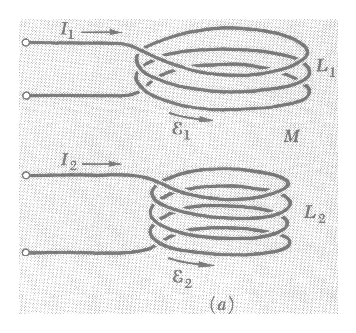
\includegraphics[width = 0.3\textwidth]{pu711a}
    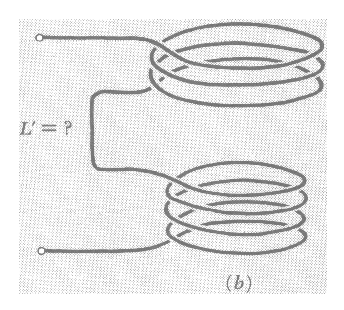
\includegraphics[width = 0.3\textwidth]{pu711b}
    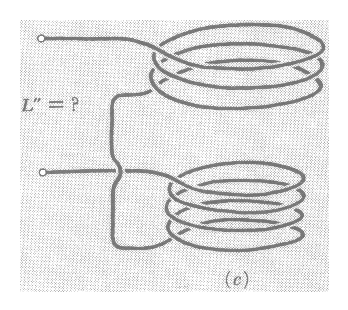
\includegraphics[width = 0.3\textwidth]{pu711c}
  \end{center}
\section{Problem \thesection: Purcell 7.18 --- Total charge flow from induced EMF}
%Scott S05 #8
  A circular coil of wire, with $N$ turns of radius $a$, is located in the field of an electromagnet.
  The magnetic field is perpendicular to the coil, and its strength has the constant value $B_{0}$ over that area.
  The coil is connected by a pair of twisted leads to an external resistance. The total resistance of this closed
  circuit is $R$. Suppose the electromagnet is turned off, its field dropping more or less rapidly to zero. Derive
  the formula for the total charge which passes through the resistor and explain why it does not depend on the rapidity
  with which the field drops to zero.
\section{Problem \thesection: Purcell 7.20 --- Magnetic field due to a loop far from the loop}
%Scott S05 #8
  Can you devise a way to use the theorem $\Phi_{21}=\Phi_{12}$ to find the magnetic
  field strength due to a ring current at points in the plane of the ring at a distance from the ring much greater than the ring radius?

  \noindent \textsc{Hint}: consider two concentric coplanar rings of radius $R_{2}$ and $R_{1}$, $R_{1}\gg R_{2}$ and evaluate the effect of a small change
  of the radius of the outer ring on $\Phi_{21}$ and $\Phi_{12}$.

  \noindent \textsc{More detailed hint}:  we wish to calculate
  the magnetic field of the small loop at the location of the large
  loop.  Since the large loop is of a radius $R_1 \gg R_2$, this will
  tell us the magnetic field of a small loop at any radius $r \gg R_2$,
  at least in the plane of the small loop. The trick here is to calculate the {\it change} in
  flux, $\Delta\Phi_B$ that occurs if we adjust the radius $R_1$ by
  some amount $\Delta R_1$.  Do this with the reciprocity theorem:
  first, work out $\delta\Phi_B$ by running the current through the big
  loop.  Reciprocity says we must get the same
  $\delta\Phi_B$ when you run the current through the small loop.
\section{Problem \thesection: Purcell 7.22 --- Spinning a charged ring}
%Scott S05 #8
  A thin ring of radius $a$ carries a static charge $q$. This ring is in a magnetic field of strength $B_0$, parallel to the ring's axis, and is supported so that it is free to rotate about that axis. If the field is switched off, how much angular momentum will be added to the ring? If the ring has mass $m$, how much angular velocity will it acquire?

  \noindent \textsc{Hint}: the variation of magnetic field induces an
  electric field along the ring, which accelerates it. The electric force creates a torque about the ring's axis.
  % an angular velocity $\omega = qB_0/2mc$.
\section{Problem \thesection: Self inductance per unit length of coaxial conductors }
%Scott S05 #8
  A transmission line consists of a pair of nested, long cylindrical
  tubes with radii $R_1$ and $R_2$:

  \begin{figure}[H]
    \centering
    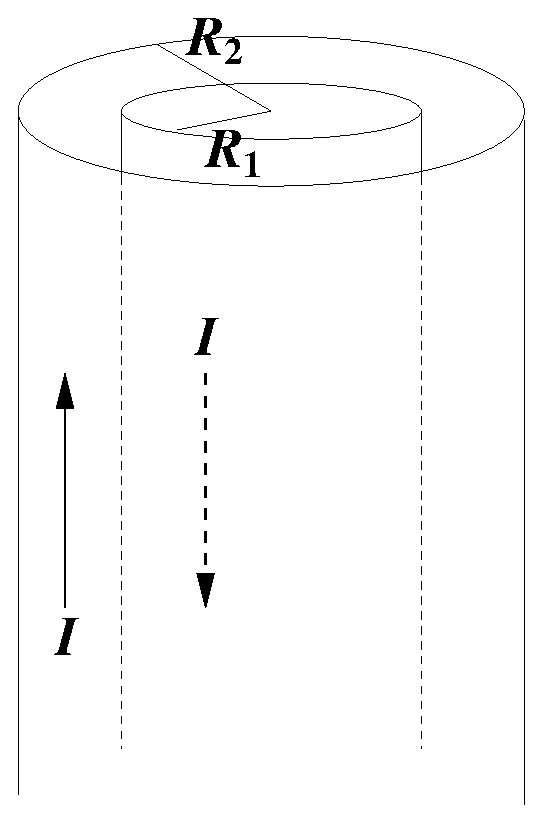
\includegraphics[width = 5cm]{coaxind}
    \label{fig:coax}
  \end{figure}

  The current $I$ flows up the outer tube and down in the
  inner tube; these currents are uniformly distributed over their
  respective surface.  Compute the self inductance per unit length of
  this configuration.

  \noindent \textsc{Hint}: make life easy for yourself and do so using
  magnetic energy.
\section{Problem \thesection: The Director's Challenge --- Extra credit!!!}
  Formulate an interesting problem that relates a topic from 8.022 to your
  intended major or any other topic about which you are passionate.  Give references
  to help future students to understand the context.  Try to give a solution.
  Any method --- theoretical, analytical, numerical, experimental --- is acceptable.
  If you can't give a full solution, outline partial solutions. Enjoy!
\end{document}
